\chapter{Applications of Probability}\label{ch:prob2}
%!TEX root = main.tex

In this chapter we go through a number of examples of the uses of probability, and present several useful mathematical tools along the way.

\section{Cancer and Probability}\label{sec:cancer_prob}

This is perhaps the most important probability question to learn, so we will spend some time covering it here and then cover it again, in a slightly different way, in Section~\ref{sec:disease} on page~\pageref{sec:disease}.  Imagine we have a population of 10000 people who have been tested for cancer, and we get the following hypothetical data:
\begin{center}
\begin{tabular}{||p{1.0in}|c|c|c||}\hline\hline
{\bf Number of Individuals}& Negative Test & Positive Test & Total\\\hline\hline
Doesn't Have Cancer& 9200  & 700 & 9900 \\\hline
Has Cancer        & 20 & 80 & 100\\\hline\hline
                           &9220 & 780 & 10000 \\ \hline\hline
\end{tabular}
\end{center}

We may be interested in a number of related probabilities.  

\example{What is the probability of both having cancer and getting a positive test for it?}

We can determine this by simply dividing the person counts from the table

\beqn
\P{cancer \textbf{and} positive test} &=& \frac{\mbox{\# of people with both cancer and positive test}}{\mbox{total \# of people}} \\
&=&\frac{80}{10000} = 0.008
\eeqn

Doing this process for every part of the table yields a posterior probability table, giving the probability for every combination of variables (i.e. with cancer and positive test, without cancer and positive test, etc...)

\begin{center}
\begin{tabular}{||p{1.0in}|c|c|c||}\hline\hline
{\bf Posterior Probability}& Negative Test  & Positive Test & Total\\\hline\hline
Doesn't Have Cancer  & 0.92  & 0.07 & 0.99 \\\hline
Has Cancer         & 0.002 & 0.008 & 0.01\\\hline\hline
                           &0.922 & 0.078 & 1.0 \\ \hline\hline
\end{tabular}
\end{center}


\example{What is the probability of both not having cancer and getting a positive test for it?}

Reading off of the table, we have 

\beqn
\P{no cancer \textbf{and} positive test} &=& 0.07
\eeqn

This question, it turns out, is a not very interesting question.  The type of question that \emph{actually} arises in life is the following,

\example{What is the probability of having cancer \emph{given} a positive test for it?}

Here we can perform the calculation in a couple of different ways, to give the (unintuitive) result.

\be
\i {\em Counting the individuals}.  


\beqn
\Pg{cancer}{positive test} &=& \frac{\mbox{\# of people with both cancer and positive test}}{\mbox{\# of people with a positive test}} \\
&=&\frac{80}{780} = 0.103
\eeqn

Although those with cancer nearly always test positive, out of the pool of all people who test positive - including a large number of false-positives - those actually having cancer are a small minority.  It is because there are many more people without cancer, so even if a small fraction of those mistakenly test positive it will outweigh the small fraction of those people with the disease.  This is why we insist on second opinions and why the rarity of a disease often matters even more than the accuracy of the test.


\i {\em Applying Product Rule}

Using the Product Rule (Section~\ref{sec:product_rule} on page~\pageref{sec:product_rule}), we have 

\beqn
\P{positive test} &=& \P{no cancer \textbf{and} positive test} + \P{cancer \textbf{and} positive test} \\
&=&= 0.07 + 0.008 = 0.078\\
\Pg{cancer}{positive test} &=& \frac{\P{cancer \textbf{and} positive test}}{\P{positive test}} \\
&=& \frac{0.008}{0.078} = 0.103
\eeqn
where we have used the sum of the \emph{Positive Test} column for $\P{positive test}$.  This is simply a shortcut to the \emph{marginalization} process (Section~\ref{sec:marginalization_intro} on page~\pageref{sec:marginalization_intro}) - determine the probability of an event by adding up all of the possible conditional situations.
\ee



\section{Weather}

\example{
If the probability that it will rain next Saturday is 0.25 and the probability that it will rain next Sunday is 0.25, what is the probability that it will rain during the weekend?
}

\subsection{First Solution - Independence}

If we assume that Sunday and Saturday weather are {\em independent} then the sum-rule (Section~\ref{sec:sumrule}) applies:

\beq
\nn\lefteqn{P(\mbox{rain Saturday {\bf or} rain Sunday})=} \\
\nn&&P(\mbox{rain Saturday}) + P(\mbox{rain Sunday}) - P(\mbox{rain Saturday {\bf and} rain Sunday}) \\
\nn&=& P(\mbox{rain Saturday}) + P(\mbox{rain Sunday}) - P(\mbox{rain Saturday})\times P(\mbox{rain Sunday}) \\
&=& 0.25 + 0.25 - 0.25\times 0.25 = 0.4375\label{eq:satsunind}
\eeq

The diagrams in Figure~\ref{fig:venn_and_or} are useful in making this calculation more intuitive, especially the term where we subtract $P(\mbox{rain Saturday})\times P(\mbox{rain Sunday})$ because otherwise we over count the double-rain weekends.  \marginnote{Another way to think of this term can be seen in answering a different question - {\em what is the total number of weekends with rain?}.  Imagine we have, in a year, 40 Saturdays with rain (by simply going through all of the Saturdays and counting them if it rains on that day)  and we also have 40 Sundays with rain.  If we want to know the number of weekends with rain we can add the Saturdays with rain and the Sundays with rain (coming to 80!) and it becomes clear that we've over counted those weekends where it rained both days - a year can only have 52 (or possibly 53) weekends.  We need to subtract those double-counts to get a reasonable answer.  The same logic applies to the calculation of probabilities.}

\subsection{Second Solution - Correlation}

Is it really reasonable that rain on Saturday and Sunday are independent events?  Probably not!  It's probably the case that knowing that it rained on Saturday, then rain on Sunday is more likely.  It may also be that if it {\em didn't rain} on Saturday then it will be {\em less likely} for rain on Sunday.  So we'd have information possibly like:
\beqn
\Pg{rain Sunday}{rain Saturday} &=& 0.35 \\
\Pg{rain Sunday}{not rain Saturday} &=& 0.15
\eeqn
Knowing this changes the equation as
\beqn
\lefteqn{P(\mbox{rain Saturday {\bf or} rain Sunday})=}\\ 
&=& P(\mbox{rain Saturday}) + P(\mbox{rain Sunday}) - P(\mbox{rain Saturday {\bf and} rain Sunday})
\eeqn
Notice, however, that we don't have a direct expression for $P(\mbox{rain Sunday})$ anymore.  We only have the {\em conditional} or {\em dependent} forms, like $\Pg{rain Sunday}{rain Saturday}$.  We can use the marginalization procedure (Equation~\ref{eq:marginalization} on page~\pageref{eq:marginalization}), and sum over all of the conditional expressions
\beqn
\P{rain Sunday}&=&\Pg{rain Sunday}{rain Saturday}\P{rain Saturday}+\\
&&\Pg{rain Sunday}{{\bf not} rain Saturday}\P{{\bf not} rain Saturday} \\
&=&0.35\times 0.25 + 0.15\times (1-0.25) =0.2
\eeqn
and then we have
\beq
\nn&=& P(\mbox{rain Saturday}) + P(\mbox{rain Sunday}) - P(\mbox{rain Saturday})\times \Pg{rain Sunday}{rain Saturday} \\
&=&0.25+0.2 - 0.25 \times 0.35 = 0.3625\label{eq:satsuncorr}
\eeq
which makes it {\em less likely} to rain on the weekend if the Sunday rain is correlated with the Saturday rain (Equation~\ref{eq:satsuncorr}) than if they are independent (Equation~\ref{eq:satsunind}).  Why is that?

One way to think of it is that, although the probability of rain on Sunday is increased due to rain on Saturday, it is more likely that Saturday is not rainy.  In those cases, which are more frequent, Sunday is less likely to be rainy as well.  When the two days are independent, Sunday's rain is the same probability regardless of Saturday's weather.   When they are dependent, then the more often clear Saturday weather makes it a little less likely for the Sunday rain, and thus lowers the chance of weekend rain by a little bit.


\section{Adding Dice}
\marginnote{
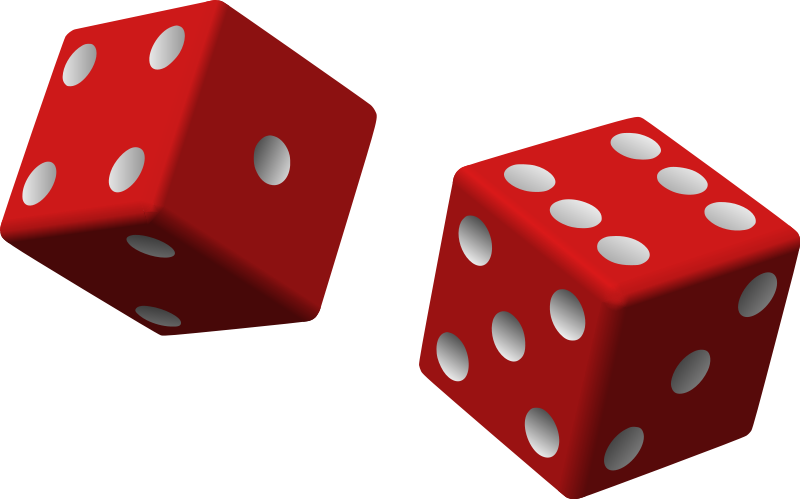
\includegraphics[width=1in]{dice/Anonymous_two_red_dice}
}
\marginnote{
All possible results from rolling two dice:

\begin{tabular}{cl}
sum & (die 1,die 2) \\ \hline
2 & (1,1) \\
3 & (1,2),(2,1)\\
4 & (3,1),(1,3),(2,2)   \\
5 & (1,4),(4,1),(3,2),(2,3)    \\
6 & (1,5),(5,1),(4,2),(2,4),(3,3)   \\
7 & (1,6),(6,1),(5,2),(2,5),(4,3),(3,4)\\
8 & (3,5),(5,3),(6,2),(2,6),(4,4)   \\
9 & (5,4),(4,5),(3,6),(6,3)    \\
10 & (4,6),(6,4),(5,5)   \\
11 & (6,5),(5,6)   \\
12 & (6,6)\\
& (36 arrangments total) 
\end{tabular}
}


\example{
What is the probability of the {\em sum} of two dice getting a particular value, say, 7?
}



In this case, we simply outline every single possibility, and count the fractions.  In a more complex case we may need to find a better method of counting, but the idea will be the same.

We find immediately that the probability of getting a sum of 7 is the largest, because there are more arrangements of the two dice which yield a sum of 7 than for any other sum.
  Each probability of a particular sum is just the number of arrangements to get that particular sum divided by the total number of arrangements of a two dice (i.e. 36). 
  
\pagebreak
\marginnote{
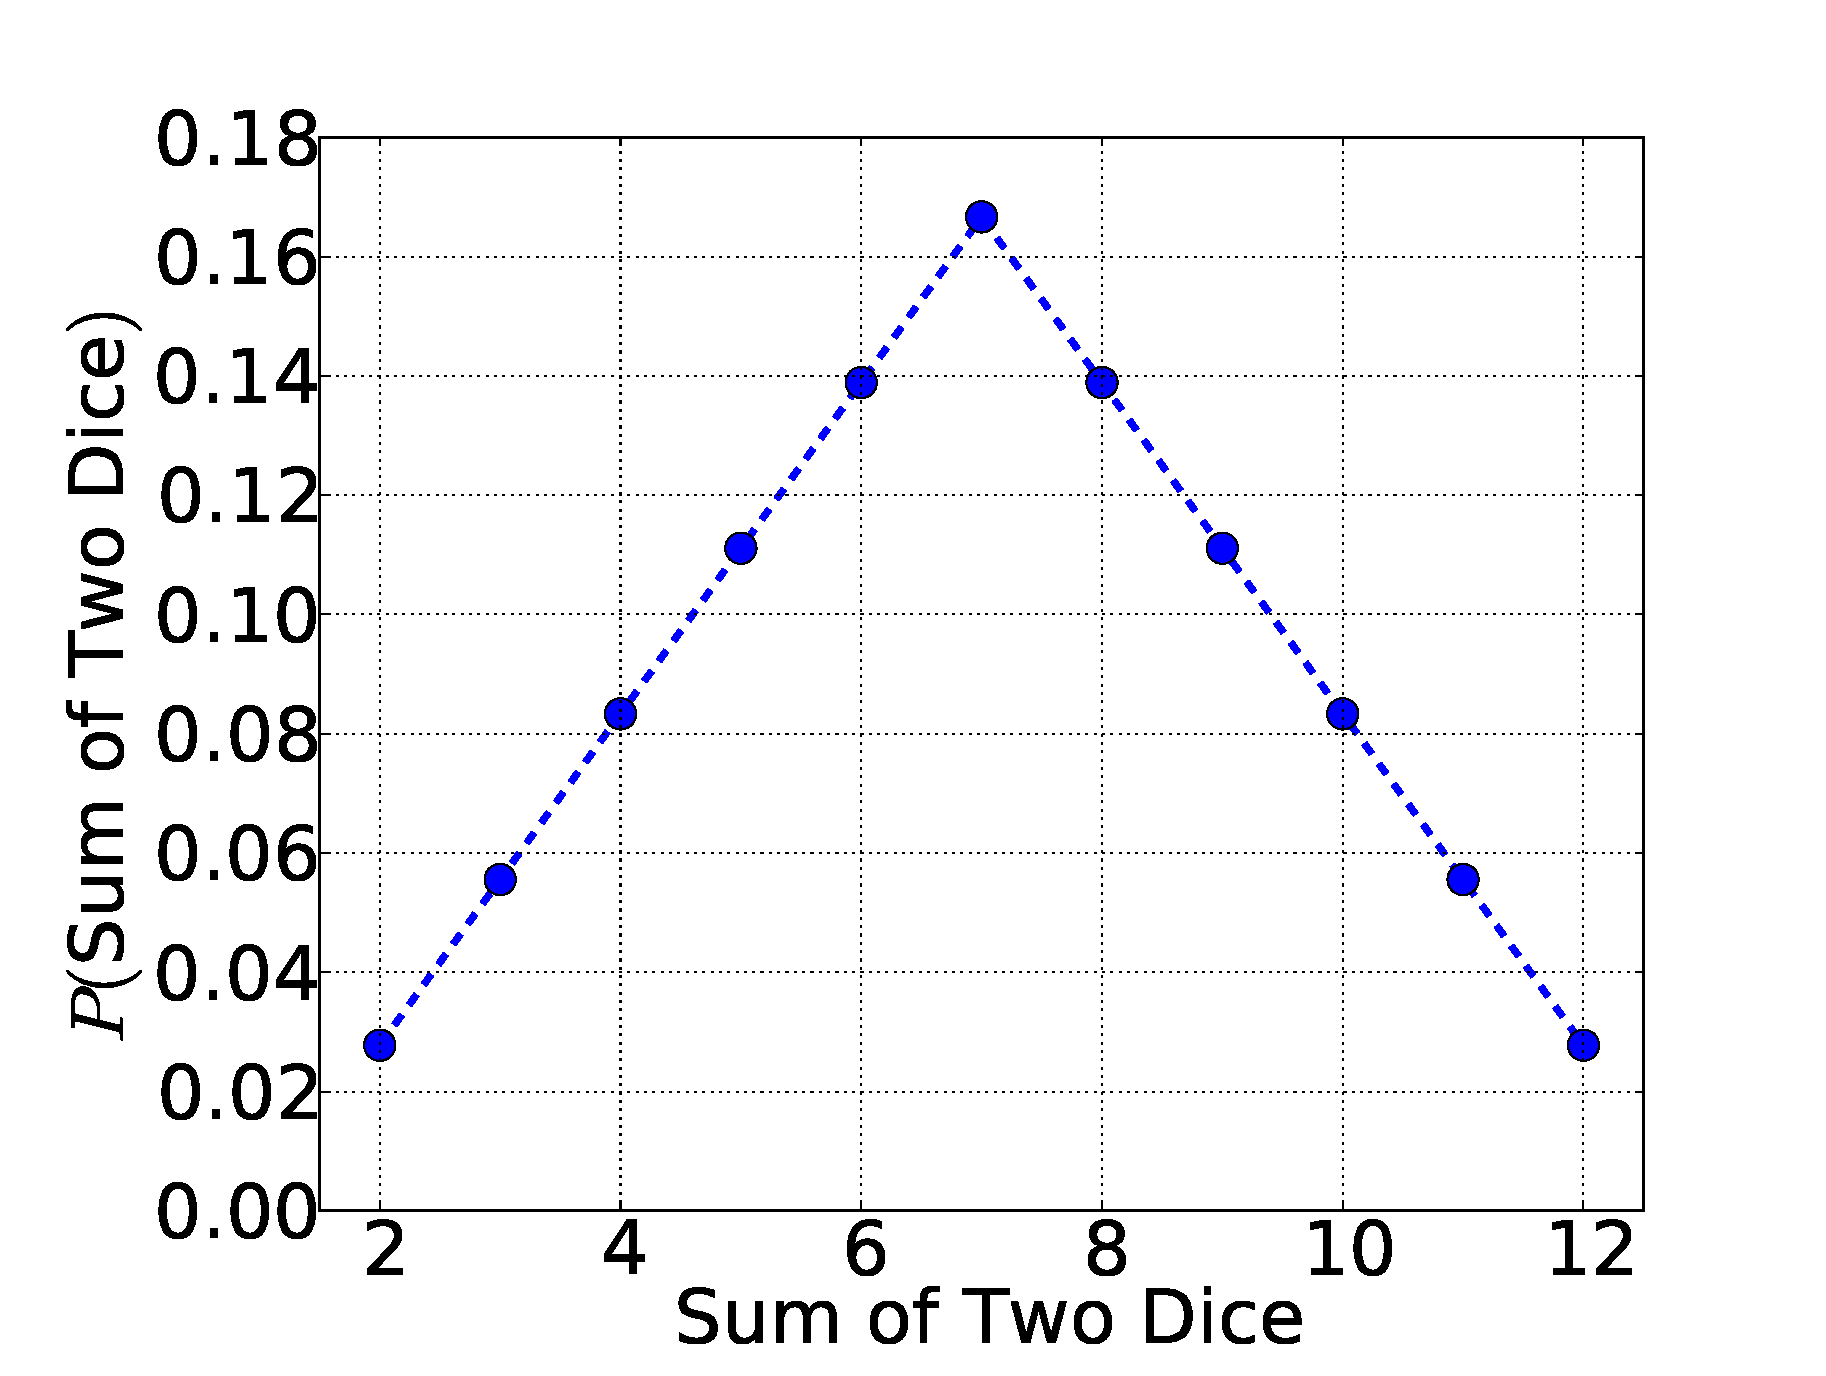
\includegraphics[width=2.2in]{sumdice2}
}
\begin{tabular}{cc}
\begin{minipage}{2in}
\beqn
P(2) &=& \frac{1}{36}=0.028 \\
P(3) &=& \frac{2}{36}=0.055 \\
P(4) &=&  \frac{3}{36}=0.083 \\
P(5) &=&  \frac{4}{36}=0.111 \\
P(6) &=&  \frac{5}{36}=0.139 
\eeqn
\end{minipage}&
\begin{minipage}{2in}
\beqn
P(8) &=&  \frac{5}{36}=0.139 \\
P(9) &=&  \frac{4}{36}=0.111 \\
P(10) &=&  \frac{3}{36}=0.083 \\
P(11) &=&  \frac{2}{36}=0.055 \\
P(12) &=&  \frac{1}{36}=0.028 
\eeqn
\end{minipage}
\end{tabular}


\example{
What is the probability of rolling a sum {\em more than 7} with two dice?
}

In our notation this is
\beqn
P(8\mbox{ or }9\mbox{ or }10\mbox{ or }11\mbox{ or }12)
\eeqn
which are all {\em exclusive events}, so we use the {\em Sum Rule} for exclusive events (Equation~\ref{eq:exclusive_sum}) and obtain
\beqn
P(8\mbox{ or }9\mbox{ or }10\mbox{ or }11\mbox{ or }12)&=&P(8)+P(9)+P(10)+P(11)+P(12) \\
&=&0.139+0.111+0.083+0.055+0.028\\
&=&0.416
\eeqn


\example{
What is the probability of rolling various sums with two dice {\em each with 20 sides}?
}
\marginnote{
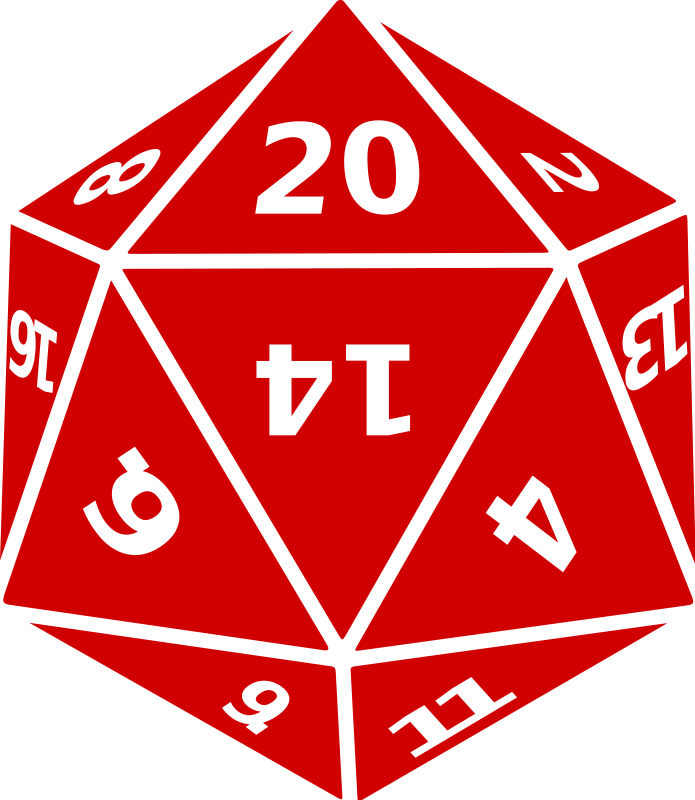
\includegraphics[width=0.5in]{dice/twenty_sided_dice}
}

20-sided dice are common in some kinds of games, and provide a nice alternative to the standard 6-sided variety.  The figure comparing the 6-sided and 20-sided dice can be see in in Figure~\ref{fig:sixandtwentysum} on page~\pageref{fig:sixandtwentysum}. 

\begin{figure*}
\begin{tabular}{cc}
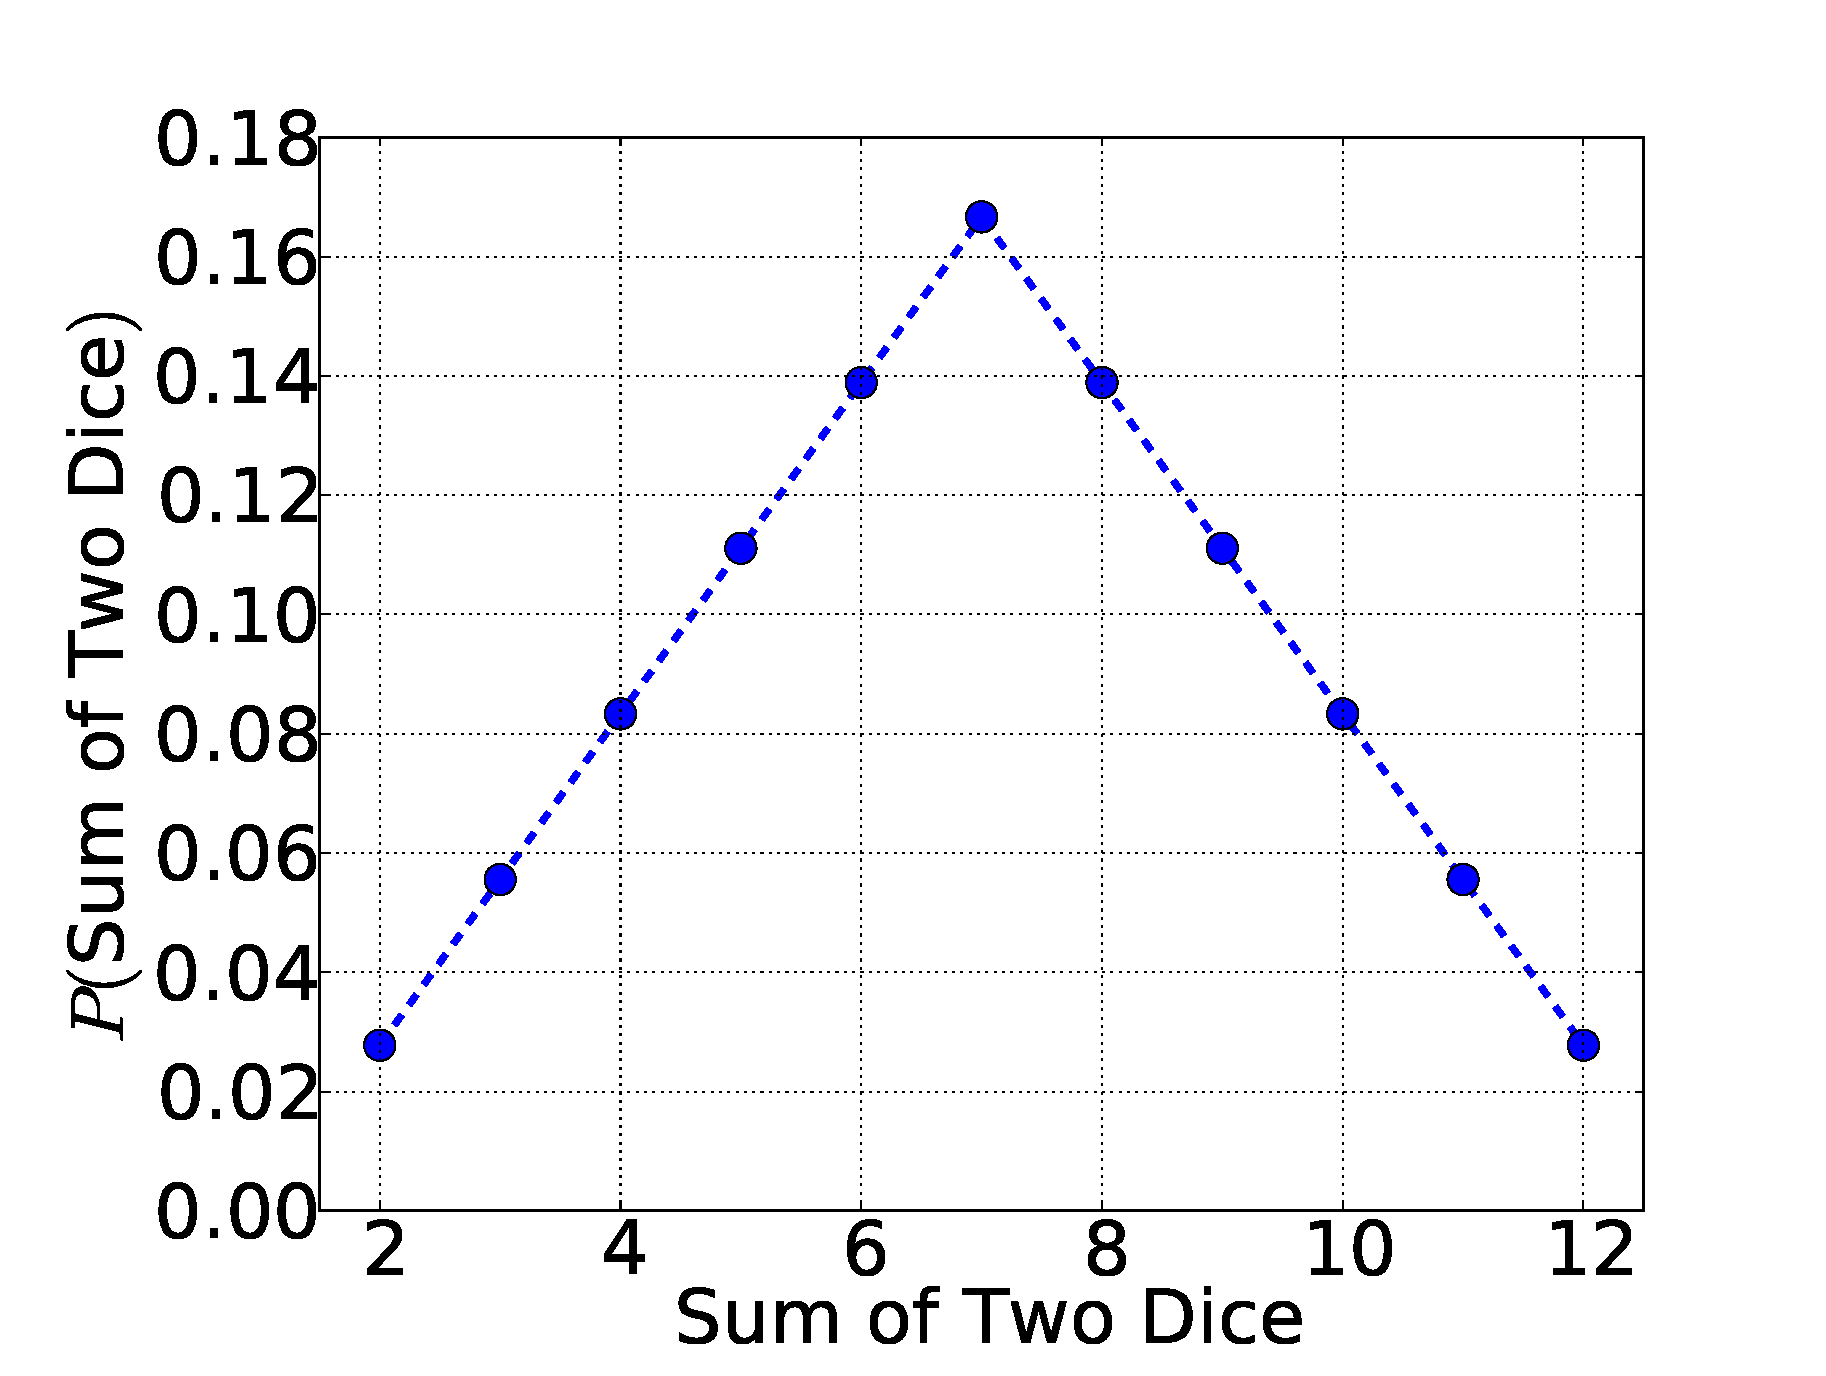
\includegraphics[width=3in]{sumdice2}&
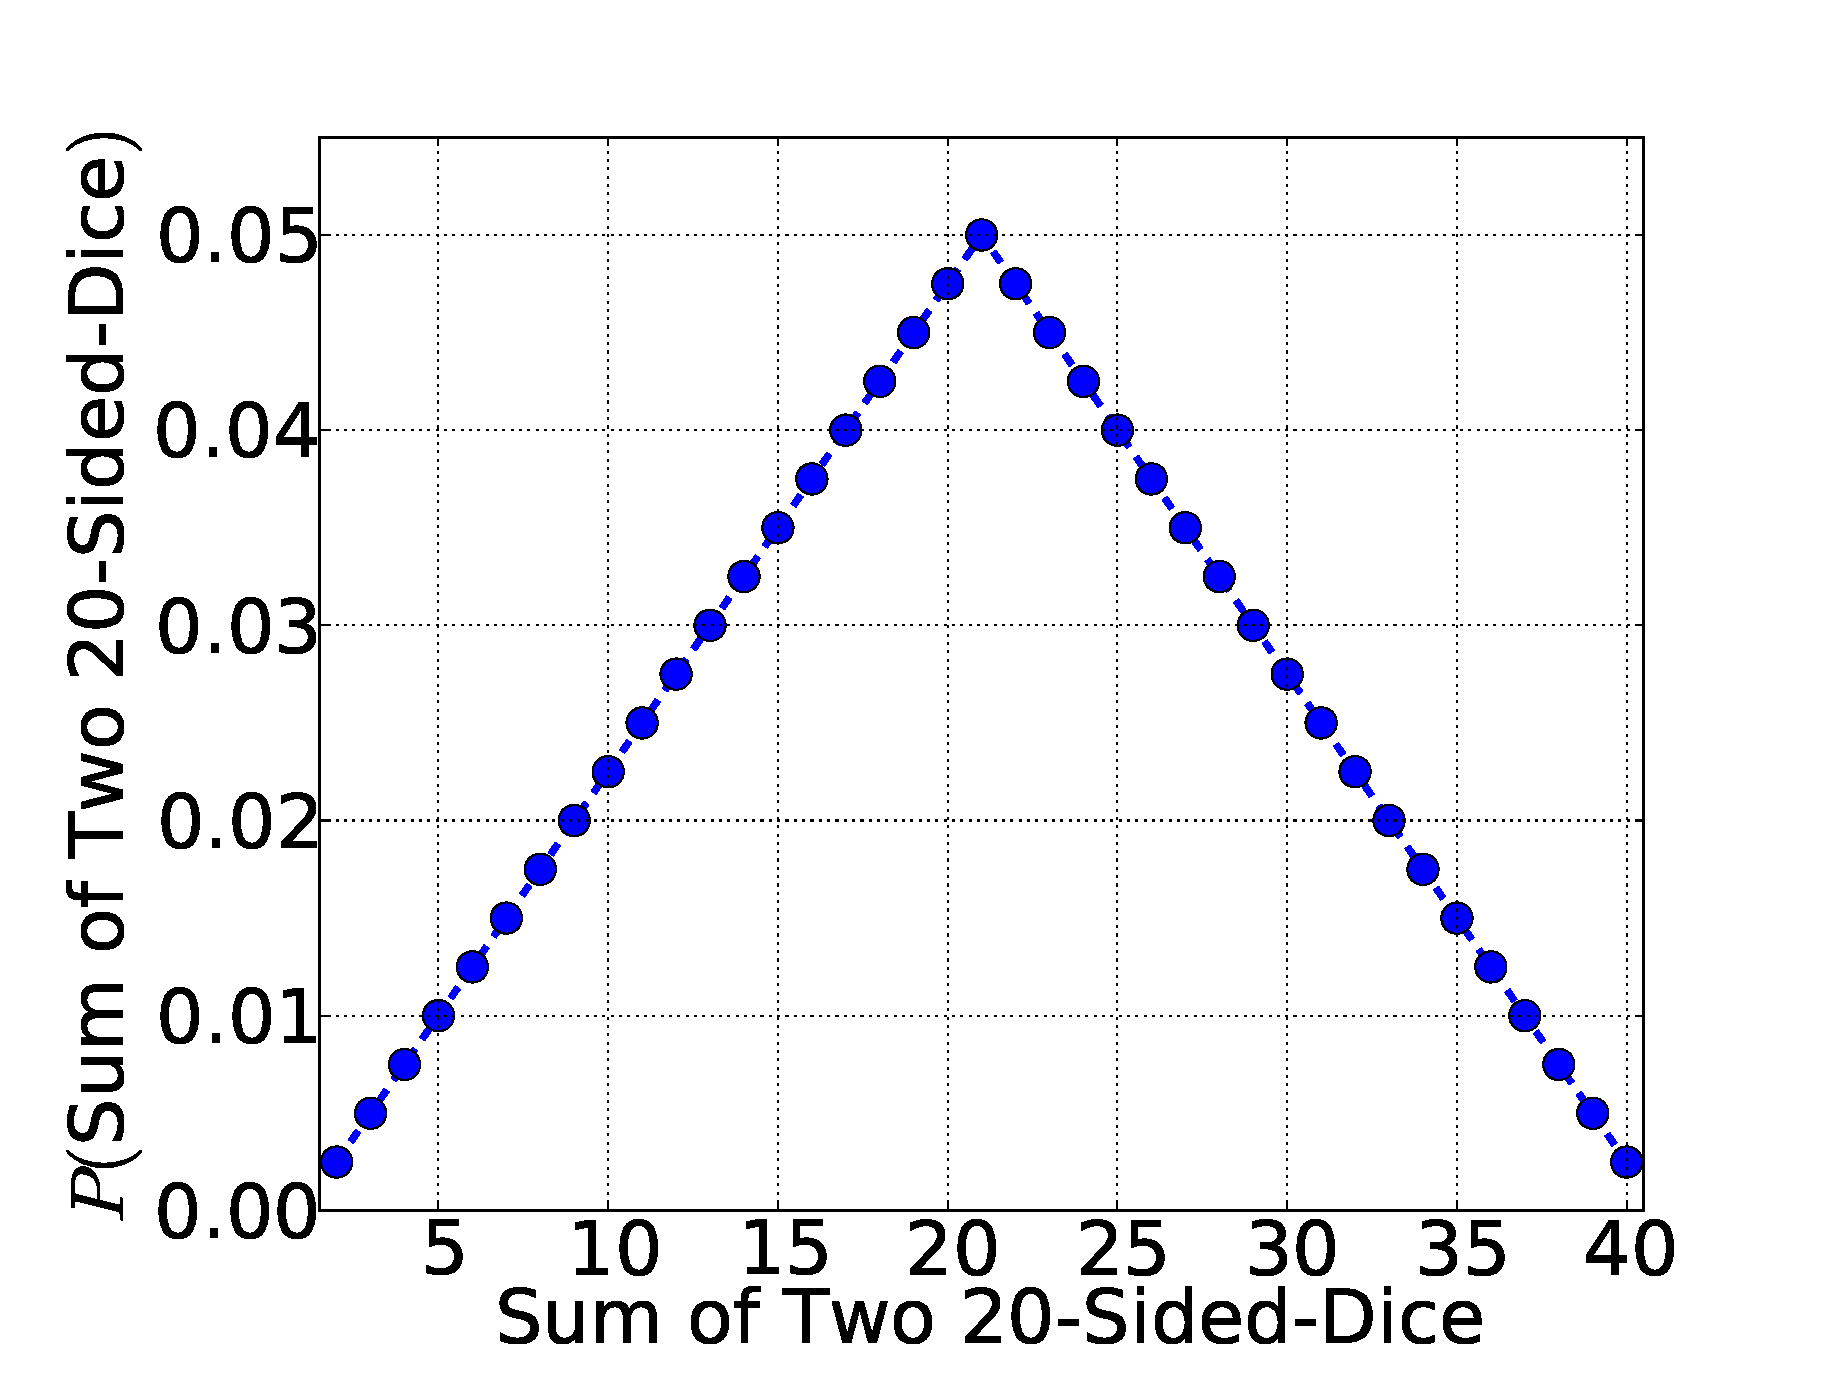
\includegraphics[width=3in]{sumdice4}
\end{tabular}
\caption{Probability for rolling various sums of two dice.  Shown are the results for two 6-sided dice (left) and two 20-sided dice (right). The dashed line is for clarity, but represents the fact that you can't roll a fractional sum, such as 2.5.}
\label{fig:sixandtwentysum}
\end{figure*}


\section{The Birthday Problem}\label{sec:birthday}

This is a famous problem in probability\cite{mosteller1965fifty}, which we address here in stages.  We introduce a simple version, and make it more complex in steps until we can tackle the general problem.

\subsection{Two People on April 3}
\example{
Let's imagine we have the case where two people meet on the street.  What is the probability that they both have April 3 as their birthday?
}

This can be solved with a straightforward application of the product rule, Equation~\ref{eq:product} on page~\pageref{eq:product}.
\beqn
A&\equiv&\mbox{Person 1 has a birthday on, say, April 3} \\
B&\equiv&\mbox{Person 2 has a birthday on, say, April 3} \\
P(A\mbox{ and }B) &=&P(A|B)P(B)
\eeqn
Each of these terms can be calculated.  Firstly, $P(A|B)$ is the probability that person 1 has a certain birthday given that person 2 has the same birthday.  However, knowing the birthday of the second person doesn't tell us anything about the birthday of the first person,  thus they are {\em independent} and $P(A|B) = P(A)$.  

Secondly, the probability of having any particular birthday is simply $P(A)=1/365$.\marginnote{This is the simplest assumption - that each day is equally likely to be born on.  However, this is probably not true - there are some days that are more likely than others.  In addition, once you start including February 29, then things obviously change.}  Finally, we have
\beqn
A&\equiv&\mbox{Person 1 has a birthday on, say, April 3} \\
B&\equiv&\mbox{Person 2 has a birthday on, say, April 3} \\
P(A\mbox{ and }B) &=&\frac{1}{365}\times \frac{1}{365} = \frac{1}{133,225}=0.0000075
\eeqn
which is extremely unlikely (see Table~\ref{table1} on page~\pageref{table1})!

\subsection{Two People}\label{subsec:twopeoplebirthday}

\example{
Two people meet on the street, and we ask what is the probability that they both have the same birthday? 
}

How is this different than the previous question, where we specified which birthday they had?  Our intuition immediately suggests that this probability must be {\em higher} than the previous one, because there are more possibilities - rather than April 3, they could be born on January 1 or May 3 or any other day.  Using our notation we have the following definitions:\marginnote{In all of these examples we are not considering leap days, which occur approximately once every four years.  These extra days do not change any of the qualitative results, and really only serve as a small extra correction to any analysis.  However, it does add a fair amount of bookkeeping with very little increase in enlightenment, so we choose to avoid this problem in our examples.}

\beqn
C_{1}&\equiv&\mbox{Person 1 and Person 2 both have a birthday on January 1} \\
C_{2}&\equiv&\mbox{Person 1 and Person 2 both have a birthday on January 2} \\
&\vdots& \\
C_{365}&\equiv&\mbox{Person 1 and Person 2 both have a birthday on December 31}
\eeqn
and the probability we are looking for is
\beqn
P(C_{1}\mbox{ or }C_{2}\mbox{ or }\cdots\mbox{ or }C_{365})
\eeqn

In this situation we can note that these are {\em exclusive} statements.  For example, it can't be true that both $C_{1}$ {\em and} $C_{2}$ are true - you can't have more than one birthday.  Thus, the Sum Rule (Equation~\ref{eq:sum} on page~\ref{eq:sum}) reduces to the Limited Sum Rule (Equation~\ref{eq:exclusive_sum}).  Further, each term in that rule is the same
\beqn
P(C_{1})=P(C_{2}) = \cdots = P(C_{365}) =\frac{1}{365}\times \frac{1}{365}
\eeqn
so we have
\beqn
\lefteqn{P(C_{1}\mbox{ or }C_{2}\mbox{ or }\cdots\mbox{ or }C_{365})=}\\
&&\underbrace{\left(\frac{1}{365}\times \frac{1}{365}\right)+\left(\frac{1}{365}\times \frac{1}{365}\right)+\cdots+\left(\frac{1}{365}\times \frac{1}{365}\right)}_{\mbox{365 terms, one for each day}}\\
&=&\frac{1}{365}=0.0027
\eeqn

Another way to think of this is to imagine that person 1 randomly ``chooses'' their birthday, $D_{1}$, and person 2 randomly ``chooses'' their birthday, $D_{2}$, and then they compare to see if the days are the same, or $D_{1}=D_{2}$.  In general, we can think of the problem broken up in this way:\marginnote{Here we find another example of the general requirement that equivalent states of knowledge give rise to equivalent probability assignments.  In this case it means that if there is more than one way to arrive at a conclusion, they each must give the same answer.  We can then choose the way that is easiest to calculate, simply out of convenience.}


\beqn
\lefteqn{P(D_{1}=D_{2}) = }\\
&&P\left(\parbox{1.5in}{$D_{1}$ is a specific day {\bf and} $D_{2}$ is the same day}\right) \times\left(\parbox{1.3in}{number of possible specific days}\right)
\eeqn

In this way, we get \beqn
P(D_{1}=D_{2}) &=& \left(\frac{1}{365}\times\frac{1}{365}\right) \times \left(365\right)\\
&=&\frac{1}{365}=0.0027
\eeqn
which is extremely unlikely (see Table~\ref{table1} on page~\pageref{table1}), but not nearly as unlikely as them both having the same April 3 birthday.

\subsection{Three People}
\example{
What is the probability that three random people have the same birthday? 
}
 Going through the same logic, we have
\beqn
P(D_{1}=D_{2}=D_{3}) &=& \left(\frac{1}{365}\times\frac{1}{365}\times\frac{1}{365}\right)\times 365\\
&=&\frac{1}{133,225}=0.0000075
\eeqn
which is even more extremely unlikely (see Table~\ref{table1} on page~\pageref{table1}) than the previous two-person example.  It is interesting to note that this is the same answer we received when we asked for the probability of two people with a {\em specific} birthday.  One can think of the three people having the same, unspecified, birthday in the following way if it helps.  The first person's birthday specifies the necessary birthday for the other two, so it is the same as the case where we specify a single birthday for two people.

\subsection{Two People...Out of Three}

Usually, we don't have a situation where we have random people meeting and all agreeing on birthdays.  What we have is a group of people talking, and two people in the group end up saying ``Hey, my birthday is April 3 too!''  This is quite a bit different, and leads to some unintuitive consequences.  Let's go through the situation with three people, and we ask the question

\example{What is the probability that {\em at least two} have the same birthday?
} \marginnote{Writing the possibilities out like this is quite tedious, and can lead to errors.  Directly after this calculation we find an equivalent, and much easier, way of writing the same calculation.  However, it is important to note that all ways of writing the same information must lead to the same answer.} Writing this out we get (somewhat messily)
\beqn
\lefteqn{P(\mbox{at least two out of three have the same birthday})=}\\
&=&P(\mbox{exactly 2 the same {\bf or} exactly 3 the same}) \\
&=&P(\mbox{exactly 2 the same})+\\
&&\underbrace{P(\mbox{exactly 3 the same})}_{\left(\frac{1}{365}\right)^{3}\times 365}-\underbrace{P(\mbox{exactly 2 {\bf and} exactly 3 the same})}_{0}
\eeqn
The term $P(\mbox{exactly 2 the same})$ can be broken up like
\beqn
P(\mbox{exactly 2 the same}) &=& P(\mbox{a specific 2 are the same}) \times \left(\parbox{.9in}{number of possibilities of 2 the same}\right)\\
&=&P(D_{1}=D_{2}\mbox{ and {\bf not} } D_{1}=D_{3})\times \left(\parbox{.9in}{number of possibilities of 2 the same}\right)
\eeqn
Applying the product rule we get\marginnote{I'm sure you're wishing for the easier way about now...it's coming in Example~\ref{ex:cleverbirthday}.}
\beqn
\lefteqn{P(\mbox{exactly 2 the same}) =}\\
&=&P(D_{1}=D_{2}\mbox{ and {\bf not} } D_{1}=D_{3})\times \left(\parbox{.9in}{number of possibilities of 2 the same}\right) \\
&=&P(D_{1}=D_{2}|\mbox{\bf not }D_{1}=D_{3})P(\mbox{\bf not }D_{1}=D_{3}) \times \left(\parbox{.9in}{number of possibilities of 2 the same}\right) \\
&=&\underbrace{P(D_{1}=D_{2})}_{\frac{1}{365}}\underbrace{P(\mbox{\bf not }D_{1}=D_{3})}_{\frac{364}{365}}\times \left(\parbox{.9in}{number of possibilities of 2 the same}\right)
\eeqn
Noting that there are 3 ways of getting a specific 2 the same\marginnote{These 3 ways are ``person 1 and 2 match'', ``person 1 and 3 match'', ``person 2 and 3 match.''}, we obtain for this single term
\beqn
P(\mbox{exactly 2 the same})&=&\frac{1}{365}\times\frac{364}{365}\times 3 
\eeqn
Putting it all together we have

\beqn
\lefteqn{P(\mbox{at least two out of three have the same birthday})=}\\
&=&P(\mbox{exactly 2 the same {\bf or} exactly 3 the same}) \\
&=&\frac{1}{365}\times\frac{364}{365}\times 3 + \left(\frac{1}{365}\right)^{3}\times 365\\
&=&0.0082
\eeqn

\example{What is the probability that {\em at least two} have the same birthday?  A clever shortcut.\label{ex:cleverbirthday}}

A clever way of rethinking this problem, which significantly reduces the calculations, is found by asking the following question: in a group of people, what is the probability that {\em none} of the people have the same birthday?  This can be approached in a step-wise fashion.  Person 1 ``chooses'' a birthday, out of 365 they have all 365 possibilities.  Person 2 ``chooses'' their birthday, with probability $P=364/365$ of {\em not} being the same as Person 1.  Person 3 now has 363 ``choices'' out of 365 to avoid both other birthdays, etc...  So the probability of using this process and getting to Person 3 and not have any overlapping birthdays is simply
\beqn
P(\mbox{none the same in 3 people}) &=& \frac{365}{365}\times\frac{364}{365}\times \frac{363}{365}
\eeqn
Now, if we're interested in the probability that at least two are the same, then this is the exact {\em opposite} of the probability that none are the same.  Using the Negation Rule (Equation~\ref{eq:negation} on page~\pageref{eq:negation}) we have

\beqn
P\left(\parbox{.9in}{none the same in 3 people}\right) + P\left(\parbox{.9in}{{\bf not} ``none the same in 3 people''}\right) &=& 1 \\
P\left(\parbox{.9in}{none the same in 3 people}\right) + P\left(\parbox{.9in}{at least 2 the same in 3 people}\right) &=& 1
\eeqn
which leads to
\beqn
P\left(\parbox{.9in}{at least 2 the same in 3 people}\right) &=& 1-P\left(\parbox{.9in}{none the same in 3 people}\right) \\
&=&1-\frac{364}{365}\times \frac{363}{365}\\
&=&0.082
\eeqn

\subsection{Two People...Out of Thirty}

\example{
When you have a group of 30 people, like students in a classroom, and you ask what the probability of finding two in the room with the same birthday, would your intuition say it is greater or less than 50\%?  
}
Many people find that their intuition suggests reasonably strongly that it would be less than 50\%.  We can now do this problem quite easily, and we find that our intuition does not match.\marginnote{We've often used our intuition to verify the result, but now we've reached a state where the problems get subtle enough that our intuition fails.  It is good to use ones' intuition on the ``easy'' problems, but now that we've established the process we can tackle problems where our intuition is not good enough to confirm a result.}  Following the same procedure as with 3 people, we imagine each person ``choosing'' their birthday with a dwindling selection as we go on to avoid ``choosing'' one that has already been taken.  The probability that no one in the room has the same birthday as any other is

\beqn
P(\mbox{none the same in 30 people}) &=& \underbrace{\frac{365}{365}\times\frac{364}{365}\times \frac{363}{365}\times\cdot\times\frac{336}{365}}_{\mbox{30 terms}}\\
&=&0.29
\eeqn

So the probability of having at least 2 people in the room having the same birthday is
\beqn
P\left(\parbox{.9in}{at least 2 the same in 30 people}\right) &=& 1-0.29\\
&=&0.71
\eeqn
which is 71\%!  Compare this likely outcome to the extremely rare outcome of having two random people having matched birthdays, from page~\pageref{subsec:twopeoplebirthday}.  See Figure~\ref{fig:birthday} to see a plot of this unintuitive observation.

\begin{figure}
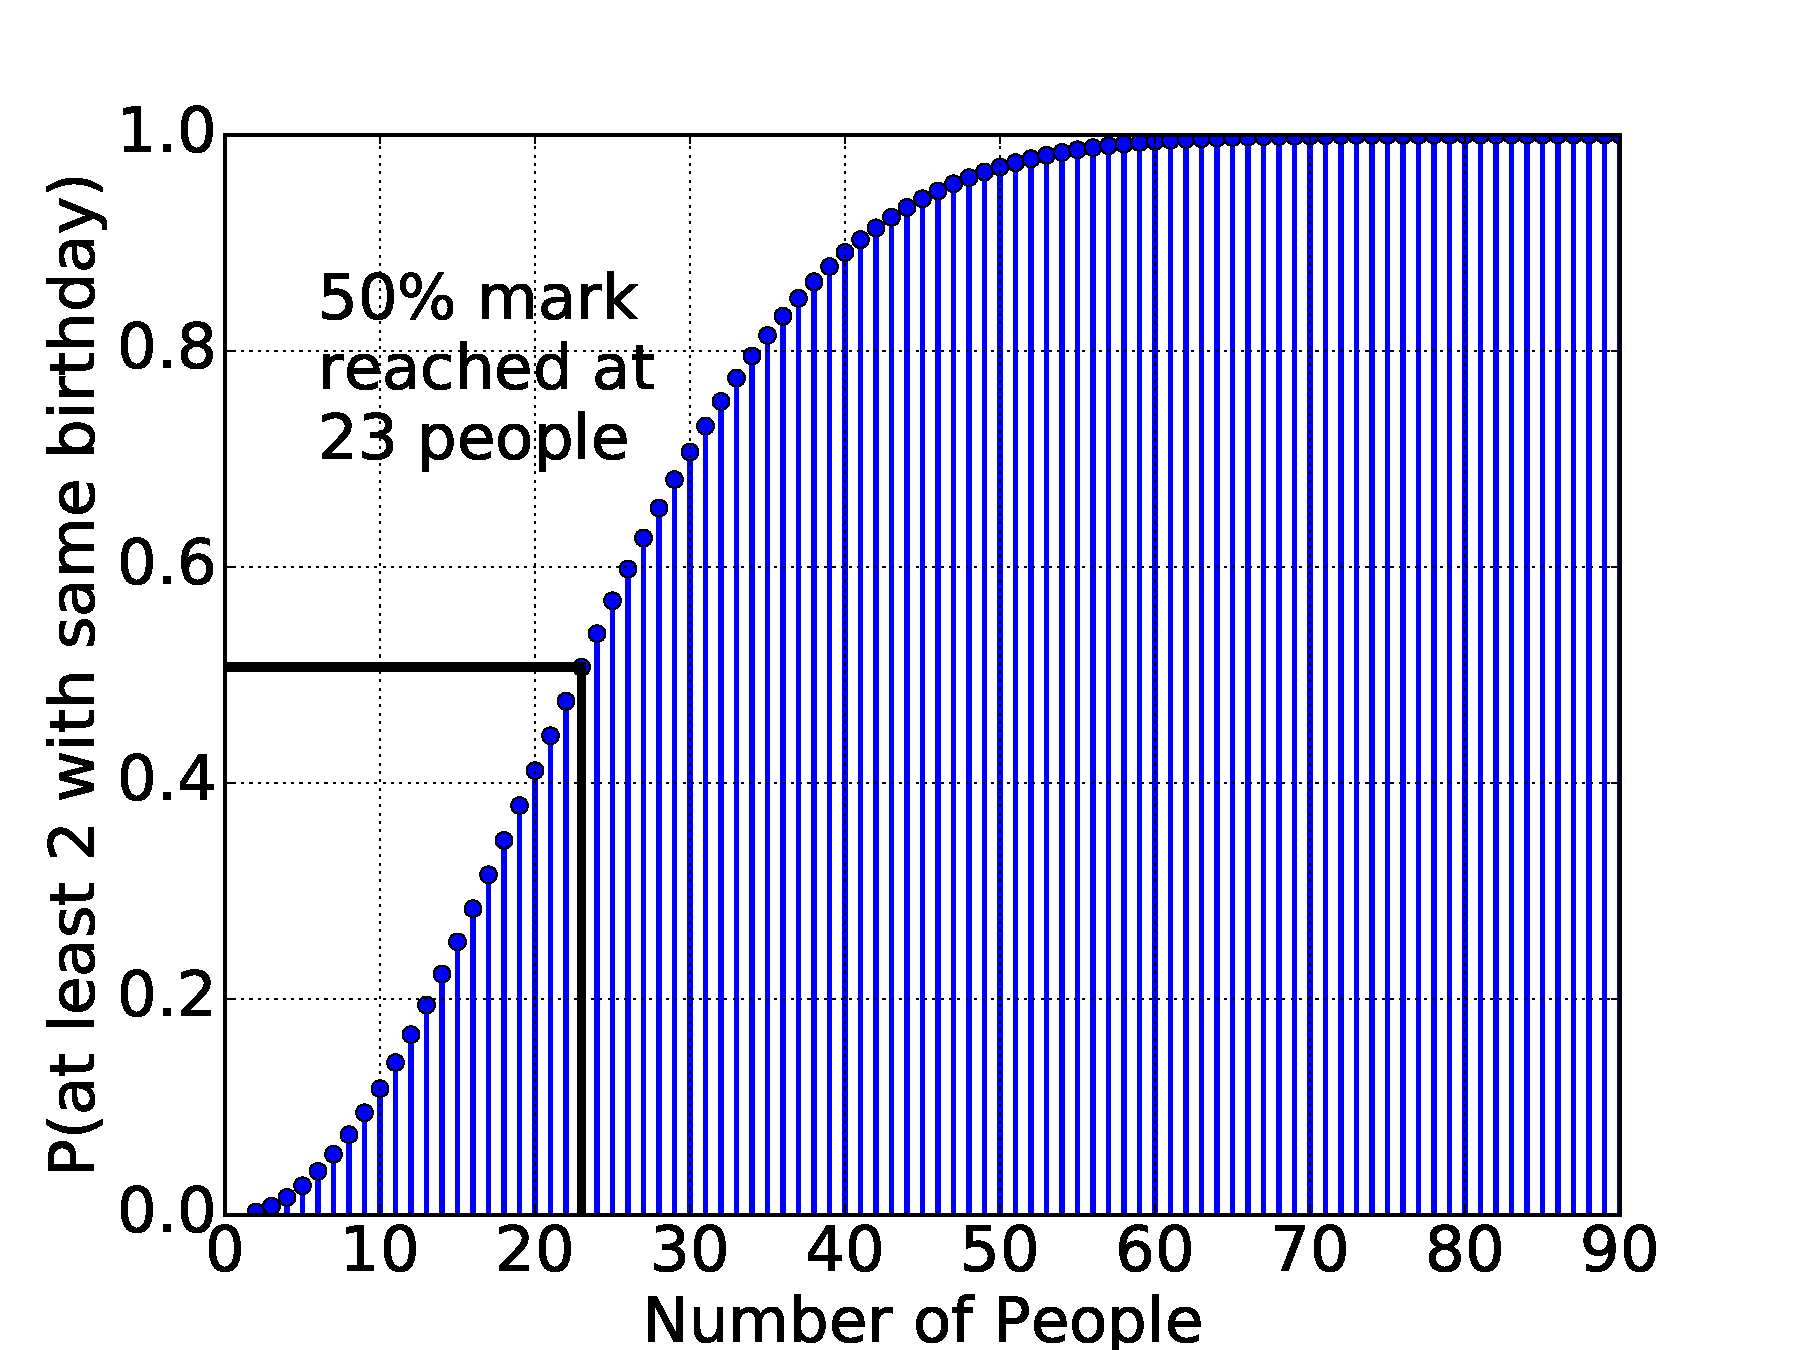
\includegraphics{birthday}
\caption{Probability of having at least two people in a group with the same birthday depending on the number of people in the group.  The 50\% mark is exceeded once the group size exceeds 23 people.}\label{fig:birthday}
\end{figure}


\section{The Lottery Problem or Rare Things Are Common}\label{sec:lottery}

This problem is identical to the birthday problem mathematically,with the only difference that the probability numbers are much smaller and the number of participants is much larger.  We start with a story about someone winning the lottery \emph{twice} in the same day!\cite{abc2002lottery}

\begin{quote}
Can you imagine winning the lottery twice in one day?

Angelo and Maria Gallina don't have to imagine - they hit twice on Nov. 20.

The married couple from Belmont, Calif., had separately bought tickets in two different California state lottery games, and both could hardly believe their eyes as all 11 winning numbers over two games came up....Before taxes, their winnings amounted to \$126,000 for the Fantasy 5 and \$17 million for the SuperLotto Plus, according to The Associated Press....Orkin arrived at the number by multiplying the roughly 41-million-to-one odds of winning the SuperLotto game and the 575,000-to-one odds of winning the Fantasy 5 game to arrive at odds of 23,575,000,000,000-to-one.
\end{quote}

%\newcommand{\E}[1]{\times 10^{#1}}
Pretty amazing!  That's something like
\beq
\P{winning two tickets}=\frac{1}{2\E{13}}\sim 5\E{-14}
\eeq
which truly is quite improbable as a single event, but is it truly an improbable event to happen \emph{somewhere}?  The assumption stated in the quote is that only two tickets were purchased.  We all know that many lottery tickets are purchased daily, which should increase the chance that \emph{somewhere} this will occur.  Even this winning couple purchased tickets every day for 20 years before winning this.

Like the birthday problem, you have to set up the problem in the negative, and as what the probability of no one winning two lotteries.  If we assume 5 million people playing daily for 20 years, this probability is:
\beq
P\left(\parbox{.7in}{no one winning two tickets}\left|\parbox{.7in}{5 million plays daily for 20 years}\right.\right)&=&\left(1-\frac{1}{2\E{13}}\right)^{5\E{6}\times 365 \times 20}\\
 \nn&\sim& (1-5\E{-14})^{5\E{6}\times 365 \times 20}\\
&=&0.998
\eeq
yielding a 0.2\% chance of this happening sometime in those 20 years - still pretty rare, but not outrageously so.  If we further imagine that this is occurring across the 50 states, this increases to 10\% chance of this happening sometime in those 20 years.  If we further imagine that there are as many as 5 different lotteries (there are usually more) that could be played per state, this jumps up to 40\%.

What we see as an initially \emph{highly} unlikely event starts to become \emph{likely} and in fact \emph{common} when considering all of the possible ways that event could be produced.



\section{Monte Hall Problem}\label{sec:monty}
One of the most popular probability problems is called the Monte Hall problem, and is based on the television game show ``Let's Make a Deal.''\cite{selvin1975problem}  It can take on many forms, but a common form is as follows\cite{vos1990ask}

\example{
Suppose you're on a game show, and you're given the choice of three doors: behind one door is a car; behind the others, goats. You pick a door, say No. 1 (but the door is not opened), and the host, who knows what's behind the doors, opens another door, say No. 3, which has a goat. He then says to you, "Do you want to change your choice to door No. 2?" Is it to your advantage or disadvantage to switch your choice, or does it matter whether you switch your choice or not?
}

The result is that {\em it is always better to switch}, where the probability of getting the car moves up from 1/3 to 2/3 by switching!
Because this problem is particularly unintuitive, we will break it up into smaller pieces.\marginnote{Most people will state that, because we are left with 2 choices, it must be 50-50.  However there is added information in the system which moves us from knowing {\em nothing} about the two choices (i.e. 50-50 chance) to knowing {\em a little bit more} about the two choices (i.e. not 50-50 chance).}   The critical aspect of this is that a {\em change in our assignment of probability to an event must be somehow tied to a change in our information about that event}.  In order to understand the problem, we must then understand where the extra information is coming from.

We will step up to the full problem listed, but for now we explore some simpler versions of the problem.
\subsection{Two Doors with Information}

\example{
Imagine we have a game with two doors: Behind one door is a car; behind the other is a goat. You pick a door, say No. 1 (but the door is not opened), and the host, who knows what's behind the doors, says that there is a 90\% chance that the car is behind door No. 2.  Is it to your advantage to switch your choice?
}

Initially there is a two-door choice, with no information about either choice, so we assign equal probabilities to the choices:  $\P{car behind No. 1}=\P{car behind No. 2}=0.5$ (i.e. a 50-50 chance).  After the host gives information, this changes.  Although this is still a two-door choice, it is no longer a 50-50 chance.  By having a knowledgable person give you information suddenly changes the situation to a 10-90 chance, and it is much better for you to switch.

What if the host were a little less direct?  Perhaps something like

\example{
The host, who knows what's behind the doors, points to a door, choosing the correct door 90\% of the time and the incorrect one 10\%.  You pick a door, say No. 1, and the host points to door No. 2. Is it to your advantage to switch your choice?
}
This amounts to an identical situation as the previous one - the host is giving you correct information 90\% of the time, and we are in a much better position switching.

\subsection{Three Doors with Information}

We return to the three-door case with a slight variation
\example{
Suppose you're on a game show, and you're given the choice of three doors: Behind one door is a car; behind the others, goats. You pick a door, say No. 1 (but the door is not opened), and the host, who knows what's behind the doors, says that another door, say No. 3, has a 0\% chance of having a car, and that the remaining door (that you haven't chosen - i.e door No. 2) has a 66\% of having the car.  He then says to you, "Do you want to pick door No. 2?" Is it to your advantage to switch your choice?
}

In this case, switching to door No. 3 would be ridiculous - we know the car isn't there, because the (honest) host knows that it is not there.  The host also has told us that there is a 66\% chance of the car behind door No. 2, and thus we have $\P{car behind No. 1}=0.34$ and $\P{car behind No. 2}=0.66$  and it is better to switch to door No. 2.

It isn't the number of choices that is important, it is the information we have about those choices.  When you have no information, we assign equal probabilities.  When we have information, we can assign non-equal probabilities.  

\subsection{Three Doors Down To Two}

Back to our original problem, we have

\example{
Suppose you're on a game show, and you're given the choice of three doors: behind one door is a car; behind the others, goats. You pick a door, say No. 1 (but the door is not opened), and the host, who knows what's behind the doors, opens another door, say No. 3, which has a goat. He then says to you, "Do you want to change your choice to door No. 2?" Is it to your advantage or disadvantage to switch your choice, or does it matter whether you switch your choice or not?}

The key part is that, no matter what happens, 
\be
\i the host {\em never} opens your door
\i the host {\em always} opens a door with a goat
\ee

\marginnote{Another way to look at this is to imagine a game with 1000 doors, car behind only one, and the host has to open up 998 doors (not yours and not the prize - if the prize is different than yours).  Once you pick, say door number 1, and the host opens every door except door 576, and gives you the opportunity to switch is it a good choice?  Of course!  Ones intuition realizes that my initial 1/1000 chance of getting it right (and thus have the other door have a goat) is swamped by the 999/1000 chance of getting it wrong, and the host being forced to open every door without the prize.}  Given that your first choice, with three equal probability choices (i.e. you have no information about any of the choices), we expect to be correct only about 33\% of the time.  If we happened to get lucky with our first choice, then the host has a pick of two doors with goats and has some freedom.  If we happened to get unlucky with our first choice (and there is a goat behind it), then the host has \emph{no freedom at all}, because there is only one remaining door with a goat.  So, about 66\% of the time the host is forced to reveal some of his information, because the door he leaves closed (other than your door) {\em must} have the car.  Thus, 66\% of the time the host is {\em telling you where the car is}, just a little indirectly. 

Formally, we need to involve model comparison, so we postpone this particular analysis until Section~\ref{sec:monty_models}. 




\newcommand{\solution}[1]{}

\section{Exercises}

\exercise{Birthdays}{
What is the probability that at least 3 people have the same birthday in a group of 50?
}
\solution{

}


\exercise{Monte Hall Again}{
Examine the case of Monte Hall with 4 doors, the host opening one door with a goat, and leaving you with a choice of 3.  Should you switch?  Does it matter which of the other two you choose?
}
\exercise{9-sided Dice}{
What is the probability of rolling various sums from two 9-sided dice?
}

\exercise{Odd Dice}{
What is the probability of rolling an odd sum with two dice?
}

\exercise{More than...}{
What is the probability of rolling more than 7 from two 20-sided dice?
}



\exercise{Cancer Questions}{
Given the table above, determine the following quantities, and describe what they {\em mean}:
\be
\i $\P{\rm cancer {\bf and} negative test}$ 
\i $\Pg{\rm cancer}{\rm negative test}$ 
\i $\P{\rm not cancer}$
\i $\P{\rm not cancer} + \P{\rm cancer}$
\ee
}


\section{Some Philosophical Applications}

\subsection{Doctors' Claims - English Language and Probability}

In Section~\ref{sec:conjunction} we introduced work by Tversky and Kahneman documenting supposed failures in proper reasoning.  In the example survey of medical internists, the internists were asked 
\begin{quote}
Which is more likely: the victim of an embolism (clot in the lung) will experience partial paralysis or that the victim will experience both partial paralysis and shortness of breath?
\end{quote}
and 91 percent of the doctors chose that the clot was less likely to cause the rare paralysis rather than to cause the combination of the rare paralysis and the common shortness of breath.  

This may not be a failure of reasoning, but a (correct!) failure of the doctors to translate the English language literally into logical language.  It is likely that when doctors are asked: ``Which is more likely: that the victim of an embolism will experience partial paralysis or that the victim will experience both partial paralysis and shortness of breath?'' they interpret it as:
\be
\i someone is {\em claiming} that the patient has an embolism
\i the patient is {\em claiming}, or someone has measured, that she has partial paralysis
\i the patient is {\em claiming}, or someone has measured, that she has shortness of breath
\ee

The doctors are separating the analysis of the \emph{claim} of the clot, which is given information, from the other claims. Another way of looking at it is to include the knowledge of the method of reporting. Someone who is reporting information about an ailment will tend to report all of the information accessible to them. By reporting only the paralysis, there are two possibilities concerning the person measuring the symptoms of the patient:
\be
\i they had the means to measure shortness breath in the patient, but there was none
\i they did not have the means to measure shortness of breath
\ee
In the first case, the doctor's probability assessment is absolutely correct: both symptoms together are more likely than just one. In the second case, the doctors are also correct: one of the sets of diagnostic results (i.e. just paralysis) is less dependable than the other set (i.e. both symptoms), thus the second one is more likely to indicate a clot or is consistent with the known clot.

It isn't that the doctors are reasoning incorrectly. They are including more information, and doing a more sophisticated inference than the strict, formal, minimalistic interpretation of the statements would lead one to do.
This analysis works well for other examples stated in the book {\em A Drunkard's Walk} by Mlodinow\citep{mlodinow2008drunkard}, like ``Is it more probable that the president will increase federal aid to education or that he or she will increase federal aid to education with funding freed by cutting other aid to states?''

All of this underscores the need to be careful translating statements of probability into plain English and vice versa.

\subsection{Diverging Opinions}

Is it possible to have people informed by the same information, and reasoning properly, to have diverging opinions?  It might seem intuitive that people given the same information, reasoning properly, would tend to come to agreement, however this is not always the case.  What is interesting is that it turns on the prior probabilities for claims.  This example comes from Jaynes, 2003\cite{Jaynes2003}.  We have the following piece of information:

\beqn
D &:=& \left\{\parbox{3in}{``Mr $N$. has gone on TV with a sensational claim that a commonly used drug is unsafe''}\right.
\eeqn
and we have observers $A$, $B$, and $C$ with different prior assignments to the reliability of Mr $N$ and of the safety of the drug.  These prior assignments may have been the result of previous inference by these observers, in a different context, or possibly due to expert knowledge.  Observers $A$ and $C$ believe, before the announcement, that the drug is reasonably safe.  Observer $B$ does not.  We have the probability assignments then:
\beqn
P_{A}({\rm Safe}) &=& 0.9 \\
P_{B}({\rm Safe}) &=& 0.1 \\
P_{C}({\rm Safe}) &=& 0.9 
\eeqn

They all agree that if the drug is not safe, then Mr $N$ would announce it, so we have
\beqn
P_{A}(D|\mbox{not Safe}) &=& 1 \\
P_{B}(D|\mbox{not Safe}) &=& 1 \\
P_{C}(D|\mbox{not Safe}) &=& 1 
\eeqn

Finally, we have the perceptions from the observers about the reliability of Mr $N$ if the drug is actually safe.  In this case, observer $A$ is trusting of Mr $N$, observer $C$ is strongly distrustful, and observer $B$ is mildly distrustful.  By ``distrustful'' we are referring to the probabilities that Mr $N$ would make the announcement that the drug is unsafe \emph{even if} the drug were actually safe.  So we have
\beqn
P_{A}(D|\mbox{Safe}) &=& 0.01 \\
P_{B}(D|\mbox{Safe}) &=& 0.3 \\
P_{C}(D|\mbox{Safe}) &=& 0.99 
\eeqn
We want to know how each observer then determines whether the drug is safe, given the announcement, or $P(\mbox{Safe}|D)$ for each observer.

Applying Bayes' Rule we have

\beqn
P_{A}(\mbox{Safe}|D)&=& \frac{P_{A}(D|\mbox{Safe})P_{A}(\mbox{Safe})}{P_{A}(D|\mbox{Safe})P_{A}(\mbox{Safe}) + P_{A}(D|\mbox{not Safe})P_{A}(\mbox{not Safe})} \\
&=&\frac{0.01 \cdot 0.9}{0.01\cdot 0.9 + 1\cdot 0.1} = 0.083
\eeqn
Following the same calculation for the others, we get the observers updating their probability assignments after the announcement, $D$, as
\beqn
P_{A}({\rm Safe}) = 0.9 &\rightarrow& P_{A}(\mbox{Safe}|D) = 0.083\\
P_{B}({\rm Safe})= 0.1 &\rightarrow& P_{B}(\mbox{Safe}|D) = 0.032 \\
P_{C}({\rm Safe}) = 0.9 &\rightarrow& P_{C}(\mbox{Safe}|D) = 0.899 
\eeqn
Observer $A$ changed their mind, Observer $B$ had their assessment confirmed a bit, and Observer $C$ barely budged.  

Although you'd think that hearing the announcement of the unsafe nature of the drug would have moved all of the probabilities by the same amount, but the information isn't that the drug is unsafe, but the someone is {\em claiming} that the drug is unsafe.  Thus, ones prior information about both the drug and who is making the claim comes into play.

\subsection{A problem of independence}

As said in the beginning of Chapter~\ref{ch:intro} (\nameref{ch:intro}), in 1968 a jury found defendant Malcolm Ricardo Collins and his wife defendant Janet Louise Collins guilty of second degree robbery.  The prosecutor focussed on the the distinctive features of the dependence, and assigned a probability to each as follows\cite{SULLIVAN:fk}:
\be
\i Partly yellow automobile 1/10
\i Man with mustache 1/4
\i Girl with ponytail 1/10
\i Girl with blond hair 1/3
\i Negro man with beard 1/10
\i Interracial couple in car 1/1000
\ee
He then followed with the calculation applying the product rule for {\em independent} events (Section~\ref{sec:independence} on page~\pageref{sec:independence}), to find the probability that \emph{all} these things could have been observed:
\beqn
\frac{1}{10}\times\frac{1}{4}\times\frac{1}{10}\times\frac{1}{3}\times\frac{1}{10}\times\frac{1}{1000} = \frac{1}{12,000,000}
\eeqn

The initial conviction was overturned for two primary reasons, one legal and one mathematical.  The legal argument was that the prosecution had not established that these initial probabilities were supported by the evidence.  However, the really devastating part of the argument was mathematical.  As you may recall, the product rule used in this way assumes the \emph{independence} of the terms (Section~\ref{sec:independence} on pageSection~\pageref{sec:independence}).  

\example{Beard and Mustache - An Examination of Independence}

For an example, the proper product rule for two of the terms above would look like:

\beqn
\lefteqn{\P{Man with beard {\bf and} Man with mustache} =}\\
&&\Pg{Man with mustache}{Man with beard}\P{Man with beard}
\eeqn

What the prosecutor was assuming is that these two items were \emph{independent}, from which it would follow that
\beqn
\lefteqn{\P{Man with beard {\bf and} Man with mustache} =}\\
&&\P{Man with mustache}\P{Man with beard}=\frac{1}{40}=0.025
\eeqn

However, with a very brief thought, we notice that this is equivalent to saying
\begin{quote}
Knowing the man has a beard tells us \emph{nothing} about the probability of him having a mustache!
\end{quote}


Clearly, it is not nearly as common to have a beard with no mustache than with one, so knowing that the man had a beard would nearly certainly imply that he had a mustache or, 

\beqn
\lefteqn{\P{Man with beard {\bf and} Man with mustache} =}\\
&&\underbrace{\Pg{Man with mustache}{Man with beard}}_{\sim 1}\P{Man with beard} \sim \frac{1}{10}
\eeqn

and the probability calculated, just from these two terms, is much higher than the prosecutor was communicating.


Similar sorts of absurdities occur with other terms, like ``blond hair'' and ``pony tail'', as well as others.  Finally, even if it was the case that this is a somewhat rare combination, given the number of people in Los Angeles, one might be able to calculate the probability that there is at least one more couple satisfying these characteristics.  Just like the lottery problem (Section~\ref{sec:lottery} on page~\pageref{sec:lottery}), it becomes likely that there are more couples in the area like this, and thus the ruling was overturned.


\subsection{Another problem with independence}

Another problem brought up in the opening of Chapter~\ref{ch:intro} (\nameref{ch:intro}) is the case of Sally Clark.  Sally Clark was convicted in 1999 of the murder of her two young sons\cite{KAY:2003uq}.  In the case, the statistical argument was
\begin{quote}
Professor Meadow was asked if a figure of 1 in 8,543 reflected the risk of there being a single SIDS within such a family. He agreed that it was. A table from the CESDI report was placed before the jury. He was then asked if the report calculated the risk of two infants dying of SIDS in that family by chance. His reply was:
`\emph{`Yes, you have to multiply 1 in 8,543 times 1 in 8,543 and I think it gives that in the penultimate paragraph. It points out that it's approximately a chance of 1 in 73 million.''
}\end{quote}

What he was doing was equating the following in the product rule (Section~\ref{sec:product_rule} on page~\ref{sec:product_rule}):
\beqn
\Pg{second child dying of SIDS}{\textbf{first} child dying of SIDS} = \P{second child dying of SIDS}
\eeqn
which is equivalent to saying
\begin{quote}
Knowing that the child dies of a [not well understood] disease tells us \emph{nothing} about the probability of the second child dying of the same [not well understood] disease.
\end{quote}
Clearly this is ridiculous, because if there is a common source to the disease, the one death certainly increases the probability of the second.  Such a common source could be something shared in the environmental or perhaps a genetic disposition in the family for the disease.


\subsection{Prosecutor's Fallacy}

Both of the cases above are examples of what is called the prosecutor's fallacy.  It occurs when someone assumes that the prior probability of an event is equal to the probability that the defendant is innocent.  A simple example is that ``if a perpetrator is known to have the same blood type as a defendant and 10\% of the population share that blood type; then to argue on that basis alone that the probability of the defendant being guilty is 90\% makes the prosecutors's fallacy, in a very simple form.''\cite{Wikipedia:2014fk}

Essentially the prosecutor is ignoring the number of people who match the rare event.  Also, although double-deaths by SIDS are rare, they are much more common than double-murders!  One really has to look at 
\beqn
\Pg{innocence}{evidence}
\eeqn
which is not the same as
\beqn
\P{evidence}
\eeqn




\section{Computer Examples}
\begin{fullwidth}
\subsection{Coin Flips}


\begin{lstlisting}
from sie import *
\end{lstlisting}

Generate a small list of data...

\begin{lstlisting}
data=randint(2,size=10)
print data
\end{lstlisting}

\begin{verbatim}
[1 0 0 1 0 0 0 1 0 0]
\end{verbatim}

Generate a slightly larger list of data...

\begin{lstlisting}
data=randint(2,size=30)
print data
\end{lstlisting}

\begin{verbatim}
[1 1 1 0 0 0 0 1 1 1 1 0 1 1 0 1 1 0 0 1 1 1 0 1 0 0 1 1 0 0]
\end{verbatim}

\begin{lstlisting}
data=randint(2,size=(2000,10))
data
\end{lstlisting}

\begin{verbatim}
array([[1, 0, 1, ..., 1, 0, 0],
       [1, 1, 1, ..., 0, 1, 0],
       [0, 0, 1, ..., 0, 0, 0],
       ..., 
       [0, 0, 0, ..., 1, 1, 0],
       [0, 1, 0, ..., 0, 1, 1],
       [0, 1, 1, ..., 1, 0, 1]])
\end{verbatim}

We have here a large collection of numbers (20000 of them!), organized in 2000
rows of 10 columns.  We can sum all of the 20000 values, or we can sum across
columns or across rows, depending on what we want.

\begin{lstlisting}
sum(data)  # add up all of the 1's
\end{lstlisting}

\begin{verbatim}
9988
\end{verbatim}

\begin{lstlisting}
sum(data,axis=0)  # sum up all of the columns
\end{lstlisting}

\begin{verbatim}
array([1011, 1010, 1001, 1051, 1001, 1008,  962,  990,  976,  978])
\end{verbatim}

\begin{lstlisting}
sum(data,axis=1)  # sum up all of the rows
\end{lstlisting}

\begin{verbatim}
array([3, 7, 3, ..., 5, 4, 6])
\end{verbatim}

Typically the hist command makes its own bins, which may not center on the
actual count values.  That's why we call countbins(N), to make bins centered on
the counts.

\begin{lstlisting}
N=sum(data,axis=1)  # number of heads in each of many flips
hist(N,countbins(10))
xlabel('Number of Heads')
ylabel('Number of Flips')
\end{lstlisting}

\begin{verbatim}
<matplotlib.text.Text at 0x10856e990>
\end{verbatim}

\begin{center}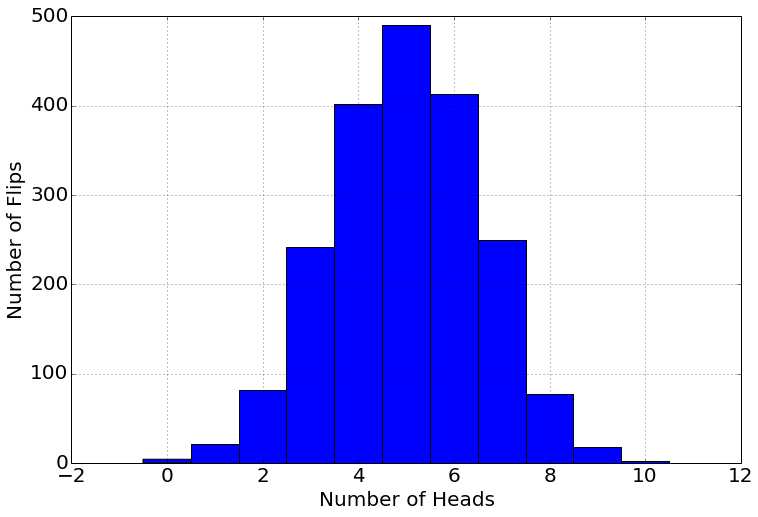
\includegraphics[width=4.5in]{Applications_of_Probability/Applications_of_Probability_fig0.png}\end{center}

To get a probability distribution, we divide the histogram result by $N$.

This distribution is Bernoulli's equation, or in other words, the binomial
distribution.

\[ p(h,10) = {10 \choose h} 0.5^h \cdot 0.5 ^{10-h} \]

\begin{lstlisting}
h=array([0,1,2,3,4,5,6,7,8,9,10])

# or...

h=arange(0,11)
\end{lstlisting}

(recall that ** is exponentiation in Python, because the caret (\^{}) was
already used for a computer-sciency role.)  The spaces in the equation below are
not needed, but highlight the three parts of the binomial distribution.

\begin{lstlisting}
p=nchoosek(10,h)* 0.5**h * 0.5**(10-h)
\end{lstlisting}

\begin{lstlisting}
hist(N,countbins(10),normed=True)
plot(h,p,'--o')
xlabel('Number of Heads, $h$')
ylabel('$p(h|N=10)$')
\end{lstlisting}

\begin{verbatim}
<matplotlib.text.Text at 0x108560290>
\end{verbatim}

\begin{center}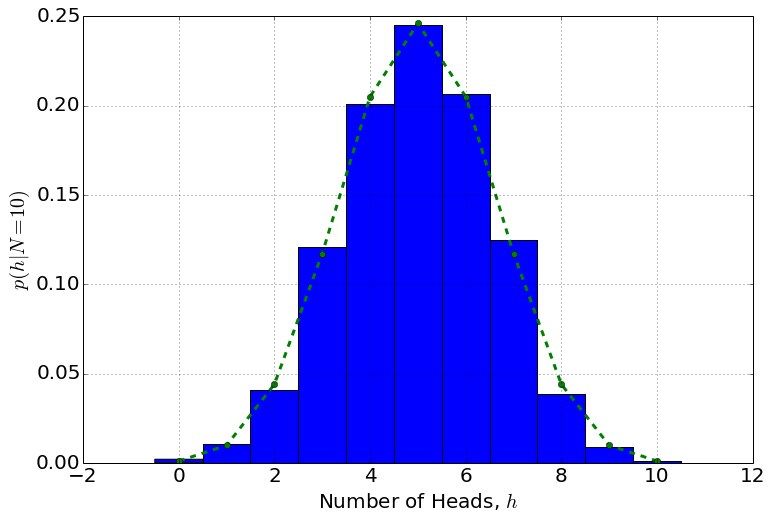
\includegraphics[width=4.5in]{Applications_of_Probability/Applications_of_Probability_fig1.png}\end{center}


\end{fullwidth}

\exercise{Simulation: 5 Heads}{
You flip a coin five times...
\be
\i What is the probability of flipping 0, 1, 2, 3, 4, and 5 heads each in these 5 flips?
\i Show in a simulation that this matches these probabilities you just found.
\ee
}



